\documentclass[11pt,a4paper]{article}
% Shared article style for handouts.
\usepackage[fontset=none]{ctex}
\usepackage{fontspec}
\setmainfont{DejaVu Serif}
\setsansfont{DejaVu Sans}
\setmonofont{DejaVu Sans Mono}
\setCJKmainfont{Noto Serif CJK SC}[BoldFont={Noto Serif CJK SC Bold}]
\setCJKsansfont{Noto Sans CJK SC}[BoldFont={Noto Sans CJK SC Bold}]
\setCJKmonofont{Noto Sans Mono CJK SC}

\usepackage[margin=1in]{geometry}
\usepackage{graphicx}
\usepackage{enumitem}
\usepackage{amsmath,amssymb}
\usepackage{booktabs,array}
\usepackage{xcolor}
\usepackage{listings}
\usepackage{tcolorbox}
\tcbuselibrary{breakable}
\usepackage{hyperref}

\definecolor{hcPrimary}{RGB}{20,72,110}
\definecolor{hcTipBG}{RGB}{239,246,252}
\definecolor{hcTipFrame}{RGB}{80,126,160}
\definecolor{hcWarnBG}{RGB}{253,244,238}
\definecolor{hcWarnFrame}{RGB}{183,84,52}
\definecolor{hcCodeBG}{RGB}{247,248,250}
\definecolor{hcCodeFrame}{RGB}{208,214,220}

\hypersetup{colorlinks=true,linkcolor=hcPrimary,urlcolor=hcPrimary,citecolor=hcPrimary}
\setlist{nosep}

\newtcolorbox{tipbox}{
  colback=hcTipBG,
  colframe=hcTipFrame,
  title=提示,
  fonttitle=\bfseries,
  boxrule=0.6pt,
  breakable
}

\newtcolorbox{warnbox}{
  colback=hcWarnBG,
  colframe=hcWarnFrame,
  title=警告,
  fonttitle=\bfseries,
  boxrule=0.6pt,
  breakable
}

\lstset{
  basicstyle=\ttfamily\footnotesize,
  backgroundcolor=\color{hcCodeBG},
  frame=single,
  rulecolor=\color{hcCodeFrame},
  numbers=left,
  numberstyle=\tiny,
  breaklines=true,
  showstringspaces=false,
  tabsize=2
}


\title{第二章：EDA工具与FPGA实践基础}
\author{数字电路入门}
\date{\today}

\graphicspath{{figures/}}

% Shell terminal style for code blocks
\lstdefinestyle{shell}{
  language=bash,
  basicstyle=\ttfamily\scriptsize\color{white},
  backgroundcolor=\color{black!90},
  frame=none,
  numbers=none,
  breaklines=true,
  showstringspaces=false,
  tabsize=2,
  aboveskip=0.5em,
  belowskip=0.5em,
  xleftmargin=0.5em,
  xrightmargin=0.5em,
  literate={\$}{{\textcolor{green!80!white}{\$}}}1
           {\~}{{\textcolor{white}{\textasciitilde}}}1,
  morecomment=[l]{\#},
  commentstyle=\color{gray!60}\itshape,
  keywordstyle=\color{cyan!80!white},
  stringstyle=\color{yellow!80!white},
}

\begin{document}
\maketitle

% ============================================================
\section{本章导读}
% ============================================================

在第一章里，我们站在远处看了一座城的轮廓——芯片是什么，系统怎么组织，产业链如何分工。上一章最后我们提到：芯片制造本身变成可重复、可组织、可协作的工业流程后，设计环节也必然发展出对应的工具链与工程方法。从本章开始，你要走进这座城，第一次真正坐在一台Linux机器前，安装工具、运行脚本、观察输出，并借助一个最小的实验获得可验证的正反馈。

很多初学者会问：为什么不先学电路原理，再碰工具？答案很简单——\textbf{即时反馈是认知杠杆}。几行RTL代码写下去，几秒钟后在波形窗口里看到信号随着代码变化，这种直接关联比硬背两章布尔代数再碰工具有效得多。本章的目标不是让你成为工具专家，而是让命令行工作方式和EDA工具链闭环变成你的``身体经验''。

这一章也不是Linux系统管理入门课，不是Verilog语法教材（那是第四章的事），更不是深入讲解EDA原理的专题。它的教学契约很明确：\textbf{先会跑通，再会解释；先会观察波形，再会设计电路；先建立工具链直觉，再追究每个参数的含义}。

全章只用一个实验——呼吸灯PWM计数器（lab1-breathing-led）——从仿真一直走到综合网表。

% ============================================================
\section{学习目标}
% ============================================================

学完本章后，你应当能够：

\begin{itemize}
  \item 独立搭建开源数字电路开发环境（Icarus Verilog + GTKWave + Yosys）
  \item 在Linux终端中完成文件导航、脚本执行和工程组织
  \item 用Icarus编译RTL和testbench，用GTKWave打开并分析波形
  \item 读懂波形中的时间轴、信号值、X/Z语义和时钟边沿行为
  \item 用Yosys对同一设计执行综合，打开并观察门级网表
  \item 区分仿真行为和综合产物之间的本质差异
  \item 理解开源工具与商业工具的能力边界
  \item 建立FPGA作为``可重配置硬件沙盘''的直觉
  \item 完成一个从RTL到综合网表的完整实验
\end{itemize}

% ============================================================
\section{为什么先跑工具？}
% ============================================================

\subsection{从「理论先行」到「工具先行」}

传统工科教育的常见模式是：先学两年数学物理，再学两年专业基础，最后才接触实际工具。这种模式对电路设计来说有一个明显的问题——你背了很多公式和定理，但从未验证过它们在一个真实系统里是否成立。你的知识停留在``我理解了''，而不是``我确认了''。

数字电路设计的一个特殊之处在于，\textbf{工具本身就是理解的一部分}。波形不是电路行为的``插图''，而是电路行为的直接呈现；综合不是RTL的``翻译练习''，而是RTL被硬件实现时的真实映射。如果你始终隔着理论和工具之间的距离去学习，你会产生一种常见的幻觉：以为自己懂了，但一动手就发现处处不对。

本章把这个顺序颠倒过来：\textbf{先让你动手跑通一个最小闭环，然后再在闭环的基础上逐层追加理论}。你不需要先理解PWM计数器的内部实现才能跑仿真——恰恰相反，看到波形里的三角波和PWM输出时，你会自然地想知道``这个三角波是怎么生成的''``占空比怎么控制亮度''，这些问题会引导你后续去深入学习。

\subsection{最小闭环}

一个完整的数字设计闭环包括：写RTL$\rightarrow$仿真$\rightarrow$看波形$\rightarrow$综合$\rightarrow$查网表$\rightarrow$上板验证。本章的主线重点放在前五个环节；上板部分只作为补充入口出现，帮助你把这条闭环和真实硬件联系起来。

这个闭环的价值不在于它短，而在于它\textbf{可复现}。一旦你跑通了一次，后续每一章的概念都可以放进同一个闭环里验证。第三章的组合逻辑可以写RTL然后看波形；第四章的Verilog语法可以边学边编译；第七章的系统级设计可以复用同样的目录结构和脚本。这个闭环是你后面所有学习的\textbf{工作台}。

% ============================================================
\section{命令行：工程师的工作台}
% ============================================================

\subsection{为什么命令行不是「更高级」，而是更务实}

如果你习惯了Windows的图形界面，第一次面对一个黑底白字的终端窗口时，可能会觉得这是一种``退步''。双击图标、拖拽文件、点击按钮，这些操作明明更直观，为什么要退回到打字输入？

这个问题问得对。图形界面的优势是\textbf{易发现性}——你不需要记忆命令，看着图标就知道能做什么。但工程工作有一个特点：\textbf{大量动作是重复的、可预测的、需要精确复现的}。你今天跑了一次仿真，明天可能要跑五十次；你在一台机器上配好了环境，需要在三台机器上复制同样的配置；你调试一个问题，需要精确记录每一步操作以便复现。

在这些场景下，图形界面的``易发现性''变成了负担：每一次点击都无法被记录、无法被脚本化、无法在不同机器间精确复现。而命令行的本质是\textbf{文本指令的序列}——你可以把它保存成脚本、放进版本控制、传给同事、在CI/CD（持续集成/持续部署，一种自动化构建和发布软件的流程）里自动执行。命令行不是``更高级''的操作方式，而是\textbf{更适合工程重复性和可复现性}的操作方式。

\begin{tipbox}
不要把命令行当成``必须掌握的黑魔法''。把它当成一种\textbf{可记录的操作日志}——你敲的每一行命令都是一条精确的操作记录，可以被保存、分享和重放。
\end{tipbox}

\subsection{文件系统：一棵倒着的树}

很多初学者在命令行里踩的第一个坑，不是命令拼错，而是\textbf{路径理解错了}。如果你对文件系统完全没有概念，这一节建议慢读。

\textbf{文件系统是一棵倒着的树}

想象你面前的电脑硬盘里存储着所有文件和文件夹。Linux用一种树状结构来组织它们——根目录 \texttt{/} 是树根，从它分出第一层目录（如 \texttt{/home}、\texttt{/usr}、\texttt{/etc}），每一层目录又可以继续包含子目录和文件，层层向下。

你的个人文件通常放在 \texttt{/home/<username>} 目录下。比如你登录系统的用户名是 \texttt{student}，你的主目录就是 \texttt{/home/student}。系统提供了一个快捷符号 \texttt{\textasciitilde}（波浪号）来代表该位置，所以 \texttt{cd \textasciitilde} 等价于 \texttt{cd /home/student}。

\textbf{两个特殊符号：\texttt{.} 和 \texttt{..}}

在Linux文件系统里，每个目录都自动包含两个特殊子目录：

\begin{itemize}
  \item \textbf{\texttt{.}}（一个点）——代表\textbf{当前目录}本身。当你在 \texttt{lab1/} 里执行 \texttt{ls .}，看到的和直接执行 \texttt{ls} 一模一样，因为 \texttt{.} 就是 ``我所在的这个地方''。
  \item \textbf{\texttt{..}}（两个点）——代表\textbf{当前目录的上级目录}。当你在 \texttt{lab1/sim/} 里执行 \texttt{cd ..}，就会退回到 \texttt{lab1/}。
\end{itemize}

这两个符号之所以重要，是因为大量命令都依赖它们来定位文件。比如：

\begin{itemize}
  \item \texttt{cd ..} ——返回上一级
  \item \texttt{cd ../..} ——返回上两级
  \item \texttt{bash ./run.sh} ——执行当前目录下的脚本（\texttt{./} 强调 ``就在当前目录里找''）
  \item \texttt{cp ../file.txt .} ——把上级目录的文件复制到当前目录
\end{itemize}

\textbf{绝对路径 vs. 相对路径}

现在来看 \texttt{bash sim/run.sh} 这个命令。在 \texttt{lab1/} 目录里执行它，首先Shell会先在当前目录下找 \texttt{sim/} 子目录，再在里面找 \texttt{run.sh}——这能成功，因为 \texttt{lab1/sim/run.sh} 确实存在。

但如果你先执行了 \texttt{cd synth/}，此时你的当前目录变成了 \texttt{lab1/synth/}。再执行同样的 \texttt{bash sim/run.sh}，Shell会去 \texttt{lab1/synth/sim/run.sh} 这个位置找——这个文件当然不存在，于是报错。

问题的根源在于：\texttt{sim/run.sh} 没有告诉系统 ``从哪里开始找''，它只是说 ``从当前位置往下找''。这种写法叫做\textbf{相对路径}——它的起点是``你当前在哪''。

\textbf{绝对路径}则不同。它从根目录 \texttt{/} 开始，完整写出每一步：

\begin{itemize}
  \item \textbf{相对路径}：\texttt{sim/run.sh} ——从当前目录开始解析，你在A目录和在B目录执行，结果不同
  \item \textbf{绝对路径}：\texttt{/home/student/project/lab1/sim/run.sh} ——从根目录开始解析，无论你在哪执行，都指向同一个文件
\end{itemize}

初学阶段，如果你不确定自己当前在哪个目录，最稳妥的办法是使用绝对路径，或者先 \texttt{cd} 到正确目录再执行相对路径。

\begin{warnbox}
终端窗口本身就会显示你当前所在的目录。看下面这个典型的终端界面——注意行首的 \texttt{user@hostname:\textasciitilde/projects/lab1\$}，其中 \texttt{\textasciitilde/projects/lab1} 就是当前路径：

\begin{lstlisting}[style=shell]
user@ubuntu:~/projects/lab1$ ls
Makefile  README.md  fpga/  rtl/  sim/  synth/  tb/
user@ubuntu:~/projects/lab1$ cd sim/
user@ubuntu:~/projects/lab1/sim$ bash run.sh
user@ubuntu:~/projects/lab1/sim$ cd ..
user@ubuntu:~/projects/lab1$
\end{lstlisting}

注意：从 \texttt{lab1} 进入 \texttt{sim/} 后，提示符变成了 \texttt{\textasciitilde/projects/lab1/sim}；用 \texttt{cd ..} 退回上级目录后，提示符又变回了 \texttt{\textasciitilde/projects/lab1}。终端一直在告诉你``你现在在哪''。
\end{warnbox}

\subsection{命令、目录与陷阱}

本节只列出你\textbf{立刻就要用到}的命令，不追求完整。遇到其他命令时，知道去哪查比一次性背下来更重要。

\begin{center}
\begin{tabular}{lll}
\toprule
\textbf{命令} & \textbf{作用} & \textbf{示例} \\
\midrule
\texttt{ls} & 列出当前目录内容 & \texttt{ls}, \texttt{ls -l} \\
\texttt{cd} & 切换目录 & \texttt{cd \textasciitilde}, \texttt{cd ..}, \texttt{cd sim/} \\
\texttt{mkdir} & 创建目录 & \texttt{mkdir my\_project} \\
\texttt{which} & 查找程序安装路径 & \texttt{which iverilog} \\
\texttt{bash} & 执行shell脚本 & \texttt{bash sim/run.sh} \\
\texttt{cat / less} & 查看文件 & \texttt{cat README.md} \\
\texttt{chmod +x} & 给脚本添加可执行权限 & \texttt{chmod +x run.sh} \\
\texttt{apt update} & 更新软件包索引 & \texttt{sudo apt update} \\
\texttt{apt install} & 安装软件 & \texttt{sudo apt install iverilog gtkwave yosys} \\
\bottomrule
\end{tabular}
\end{center}

\textbf{两个高频陷阱}

\begin{warnbox}
\textbf{Ctrl+C} 在终端里是\textbf{终止当前进程}，不是``复制''。终端里的复制粘贴通常是 \texttt{Ctrl+Shift+C} / \texttt{Ctrl+Shift+V}。这个坑几乎每个人都会踩一次——踩过之后记住就好。
\end{warnbox}

\begin{warnbox}
如果命令报错"command not found"，先运行 \texttt{which \textless{}command\textgreater{}}。如果返回空，说明工具没装或不在 \texttt{PATH} 里。安装前务必先执行 \texttt{sudo apt update}，否则可能装到旧版本或找不到包。
\end{warnbox}

\textbf{工程目录结构}

第一次进入lab1-breathing-led目录，会看到这样一个结构：

\begin{lstlisting}[style=shell]
lab1-breathing-led/
├── rtl/          # RTL 源文件——你设计的电路
├── tb/           # 测试平台——验证电路的代码
├── sim/          # 仿真脚本和产物
├── synth/        # 综合脚本和网表
├── fpga/         # FPGA 板级约束
└── README.md     # 实验说明
\end{lstlisting}

这个结构不是随意安排的。\texttt{rtl/} 和 \texttt{tb/} 里的文件是\textbf{源文件}——你写的、需要版本控制的；\texttt{sim/} 和 \texttt{synth/} 里的产物是\textbf{生成文件}——工具输出的、不需要版本控制的。两者分开，避免你在修改设计时不小心编辑了生成文件。

每个文件的作用：
\begin{itemize}
  \item \texttt{rtl/breathing\_led.v} : PWM呼吸灯核心电路
  \item \texttt{rtl/top.v} : Basys3顶层封装（管脚映射、按键、复位）
  \item \texttt{tb/tb\_breathing\_led.v} : 测试平台，给电路输入激励
  \item \texttt{sim/run.sh} : 一键仿真脚本，编译$\rightarrow$运行$\rightarrow$打开波形
  \item \texttt{synth/run.sh} : 一键综合脚本，运行Yosys
  \item \texttt{fpga/basys3.xdc} : 引脚约束文件（RTL端口$\leftrightarrow$物理引脚）
  \item \texttt{fpga/run.tcl} : Vivado实现脚本（综合$\rightarrow$布局布线$\rightarrow$比特流）
  \item \texttt{fpga/program.tcl} : Vivado编程脚本（下载比特流到Basys3）
  \item \texttt{Makefile} : 顶层编排：\texttt{make sim}、\texttt{make synth}、\texttt{make clean}
\end{itemize}

\begin{tipbox}
短文件用 \texttt{cat} 看（如 \texttt{cat README.md}），长文件用 \texttt{less} 看（按 \texttt{q} 退出）。按 \texttt{Tab} 键可以自动补全命令和文件名——这是减少拼写错误最有效的习惯。
\end{tipbox}

\textbf{更多命令：知道它们存在就够了}

以下命令本章不做主线要求，但你应该知道他们存在，遇到问题时知道去哪查：

\begin{itemize}
  \item \texttt{find} : 按文件名搜索（如 \texttt{find . -name "*.v"}）
  \item \texttt{grep} : 在文件内容里搜关键词（如 \texttt{grep "counter" rtl/*.v}）
  \item \texttt{cp / mv / rm} : 复制、移动、删除
  \item \texttt{\textgreater{}}（重定向）和 \texttt{|}（管道）: 把命令输出保存到文件或传给下一个命令
  \item \texttt{tmux} : 终端复用，管理远程长任务（后续章节会用到）
\end{itemize}

\begin{tipbox}
\textbf{延伸阅读：}如果你想更系统地学习Linux，推荐阅读《Getting Started Handout》中的\href{https://github.com/ZangXuanyi/getting-started-handout/blob/main/book3/01-shell-101.tex}{终端101}和\href{https://github.com/ZangXuanyi/getting-started-handout/blob/main/book3/02-linux.tex}{开始使用Linux}两章。
\end{tipbox}

% ============================================================
\section{仿真初体验：代码第一次变成波形}
% ============================================================

\subsection{一条数据流上的三个角色}

仿真不是``点一个按钮然后看结果''那么简单——它是一条由多个工具组成的流水线。理解这条流水线的意义在于：某一步出错时，你能判断问题出在编译阶段、运行阶段还是显示阶段，而不是对着黑屏干瞪眼。

\begin{enumerate}
  \item \textbf{Icarus Verilog（\texttt{iverilog}）} : 编译器。读入 \texttt{.v} 文件，输出可执行文件。相当于把Verilog代码翻译成仿真器能运行的二进制。
  \item \textbf{VVP} : 运行时引擎。执行编译产物，按testbench里的指令推进仿真时间，生成波形文件。
  \item \textbf{GTKWave} : 波形查看器。打开波形文件，把时间轴和信号值可视化。
\end{enumerate}

数据流：\texttt{.v 文件} $\xrightarrow{\text{iverilog}}$ \texttt{可执行文件} $\xrightarrow{\text{vvp}}$ \texttt{.vcd 波形} $\xrightarrow{\text{GTKWave}}$ \texttt{屏幕}

\subsection{跑通第一条命令链}

\begin{lstlisting}[style=shell]
$ iverilog -o sim/tb.vvp rtl/breathing_led.v tb/tb_breathing_led.v
$ vvp sim/tb.vvp
$ gtkwave sim/tb.vcd
\end{lstlisting}

第一步编译时，\texttt{-o sim/tb.vvp} 指定输出文件名为 \texttt{sim/tb.vvp}（而不是默认的 \texttt{a.out}）。第二步运行时，\texttt{vvp} 执行这个文件，testbench里的 \texttt{\$dumpfile("tb.vcd")} 和 \texttt{\$dumpvars(...)} 语句告诉仿真器把信号变化记录到 \texttt{tb.vcd}。第三步，GTKWave打开这个波形文件。

这里不需要你理解 \texttt{\$dumpfile} 和 \texttt{\$dumpvars} 的语法细节——第四章会系统讲 Verilog。现在只需要知道：testbench 里的这两行代码负责让仿真器``把波形存进文件''，这样 GTKWave 才能打开它。

% ============================================================
\subsection{波形里能看到什么}

波形文件可以理解成一份按时间排列的信号记录。它不是电路图，也不是最终结论；它回答的是：在仿真的每一个时刻，每根线是什么值，什么时候变，和哪些事件一起变。

打开GTKWave时，右侧横轴是时间，纵向每一行是一根信号。对本章来说，先把注意力放在三类信息上：

\begin{itemize}
  \item \textbf{当前值}：某个时刻，信号是 \texttt{0}、\texttt{1}、\texttt{X} 还是 \texttt{Z}。
  \item \textbf{变化时刻}：信号在哪些时间点改变；是每个时钟周期都变，还是隔很多周期才变。
  \item \textbf{前后关系}：某个输出变化之前，是否有输入、计数器、模式位或时钟边沿先发生变化。
\end{itemize}

因此，看波形的重点不是“这张图好不好看”，而是能不能用它复述电路行为：复位什么时候结束，计数器什么时候开始数，输出为什么在这个时刻翻转。如果这些问题答不上来，即使仿真命令没有报错，验证也还没有完成。

\subsection{第一次打开波形，先看什么}

第一次打开波形时，不要把所有信号一次性加入窗口。信号越多，越容易失去主线。比较稳妥的顺序是：

\begin{enumerate}
  \item \textbf{先看时间尺度}：按 \texttt{f}（Zoom to Fit）看完整仿真范围，再放大到几个时钟周期。先知道自己是在看全局趋势，还是在看局部细节。
  \item \textbf{再看 \texttt{clk} 和 \texttt{rst\_n}}：确认时钟确实在翻转，复位确实从有效状态释放到无效状态。时钟不动、复位不释放，后面的信号解释都不可靠。
  \item \textbf{然后看驱动信号}：例如本实验里的 \texttt{duty}、\texttt{pwm\_cnt} 和 \texttt{mode}。它们是解释输出变化的原因。
  \item \textbf{最后看输出信号}：例如 \texttt{pwm\_out}。不要只问“它有没有变”，还要问“它是不是按前面那些信号的变化而变”。
\end{enumerate}

这个顺序的好处是，它把波形阅读从“盯着线看”变成“沿着因果链检查”：先确认时间和复位，再确认内部状态，最后解释输出。后面调试更复杂的电路时，这个顺序仍然适用。

\subsection{四种常见取值}

数字仿真中只有四种基本取值：

\begin{center}
\begin{tabular}{clp{8cm}}
\toprule
\textbf{值} & \textbf{含义} & \textbf{何时出现} \\
\midrule
\texttt{0} & 逻辑低 & 正常运行 \\
\texttt{1} & 逻辑高 & 正常运行 \\
\texttt{X} & 未知 & 未初始化寄存器、仿真初始阶段、多驱动冲突 \\
\texttt{Z} & 高阻态 & 三态总线、未驱动引脚 \\
\bottomrule
\end{tabular}
\end{center}

这里最容易误解的是 \texttt{X}。\texttt{X} 的意思不是“电路里真的存在第三种稳定逻辑电平”，而是：\textbf{在当前仿真模型和当前时刻下，仿真器无法确定这个信号究竟是 0 还是 1。}

在初学阶段，你可以先把 \texttt{X} 理解成“仿真器现在无法确定这是 0 还是 1”。常见原因包括：

\begin{itemize}
  \item \textbf{仿真刚开始，寄存器还没初始化}。就像你刚打开一台电脑，内存里的值是随机的。仿真器也一样，刚启动时所有存储单元默认都是 X，直到完成复位或被赋予确定值。
  \item \textbf{代码里人为写了 X}。有时设计者故意用 X 表示“这个值我不关心”或“这个状态不应该出现”。比如在 testbench 里初始化某个信号为 X，看它后面会不会被正确赋值。
  \item \textbf{两条线同时控制一个信号，给的值还不一样}。比如一条线说“这是 0”，另一条线说“这是 1”，仿真器无法裁决，只能显示 X。这通常是设计错误。
\end{itemize}

因此，一个更稳妥的判断是：\textbf{在复位尚未完成、仿真刚开始的阶段，出现 \texttt{X} 并不奇怪；但在设计进入你期望的正常工作阶段后，如果关键控制信号上仍然持续出现 \texttt{X}，通常就值得警惕。} 先不要把每一个 \texttt{X} 都当成灾难，但也绝不要把它当空气。

\texttt{Z} 则表示高阻态，常见于三态总线或暂时无人驱动的引脚。对本章实验来说，你更常见的是 \texttt{0}/\texttt{1} 和偶尔需要解释清楚的 \texttt{X}；\texttt{Z} 先知道它是什么即可。

\subsection{组合逻辑 vs. 时序逻辑在波形上的区别}

\textbf{组合逻辑}关心的是“当前输入决定当前输出”。在 RTL 仿真里，你经常会看到输入一变，输出也几乎立刻跟着变。这并不意味着真实硬件完全没有延迟，而是因为本章看到的是较理想的功能级仿真，很多物理延迟细节还没有被展开。

\textbf{时序逻辑}（寄存器）则不同。它不是“输入一变输出就跟着变”，而是要等到时钟边沿才更新状态。对初学者来说，最重要的观察不是去凭肉眼诊断复杂时序问题，而是先建立一个稳定直觉：

\begin{itemize}
  \item 时钟边沿像“拍照时刻”
  \item 寄存器在这些离散时刻更新自己的状态
  \item 两个边沿之间，寄存器保存的是上一次采样得到的结果
\end{itemize}

所以你在波形里最该看的，是“某个状态信号是不是总在时钟边沿附近发生更新”，而不是把所有边沿附近的细小变化都直接解释成建立时间或保持时间问题。那些更正式的时序概念，会在后面章节系统展开。

\subsection{呼吸灯的波形长什么样}

在 GTKWave 中，建议先添加这三个信号：
\begin{itemize}
  \item \texttt{duty} : 占空比参考值
  \item \texttt{pwm\_cnt} : PWM 载波计数器
  \item \texttt{pwm\_out} : 最终输出到 LED 的 PWM 信号
\end{itemize}

这里有一个很重要的上下文：\textbf{testbench 里为了让仿真更快，把参数缩小了。} 也就是说，你在波形里看到的不是板上真实运行时那组很大的计数范围，而是一个“缩微版”的呼吸灯。

因此，在本章的仿真波形里，你更应该抓住的是\textbf{形状关系}，而不是死记具体数字：

\begin{itemize}
  \item \texttt{duty} 会先上升、再下降，形成一个三角波式的变化趋势
  \item \texttt{pwm\_cnt} 会快速循环计数，形成锯齿波
  \item \texttt{pwm\_out} 的高电平宽度会跟着 \texttt{duty} 改变：\texttt{duty} 小时脉冲窄，\texttt{duty} 大时脉冲宽
\end{itemize}

这三者之间的关系，才是你真正要看懂的内容：\texttt{pwm\_out} 不是凭空变化，而是比较器根据 \texttt{pwm\_cnt < duty} 这个条件生成的结果。

\begin{tipbox}
先按 \texttt{f}（Zoom to Fit）看完整变化趋势，再放大到几个时钟周期，观察 \texttt{pwm\_cnt} 和 \texttt{pwm\_out} 的对应关系。一个看``整体趋势''，一个看``局部机制''，两种尺度都要会用。
\end{tipbox}

下图是一张实际的 GTKWave 截图。让我们逐个信号看过去：

\begin{center}
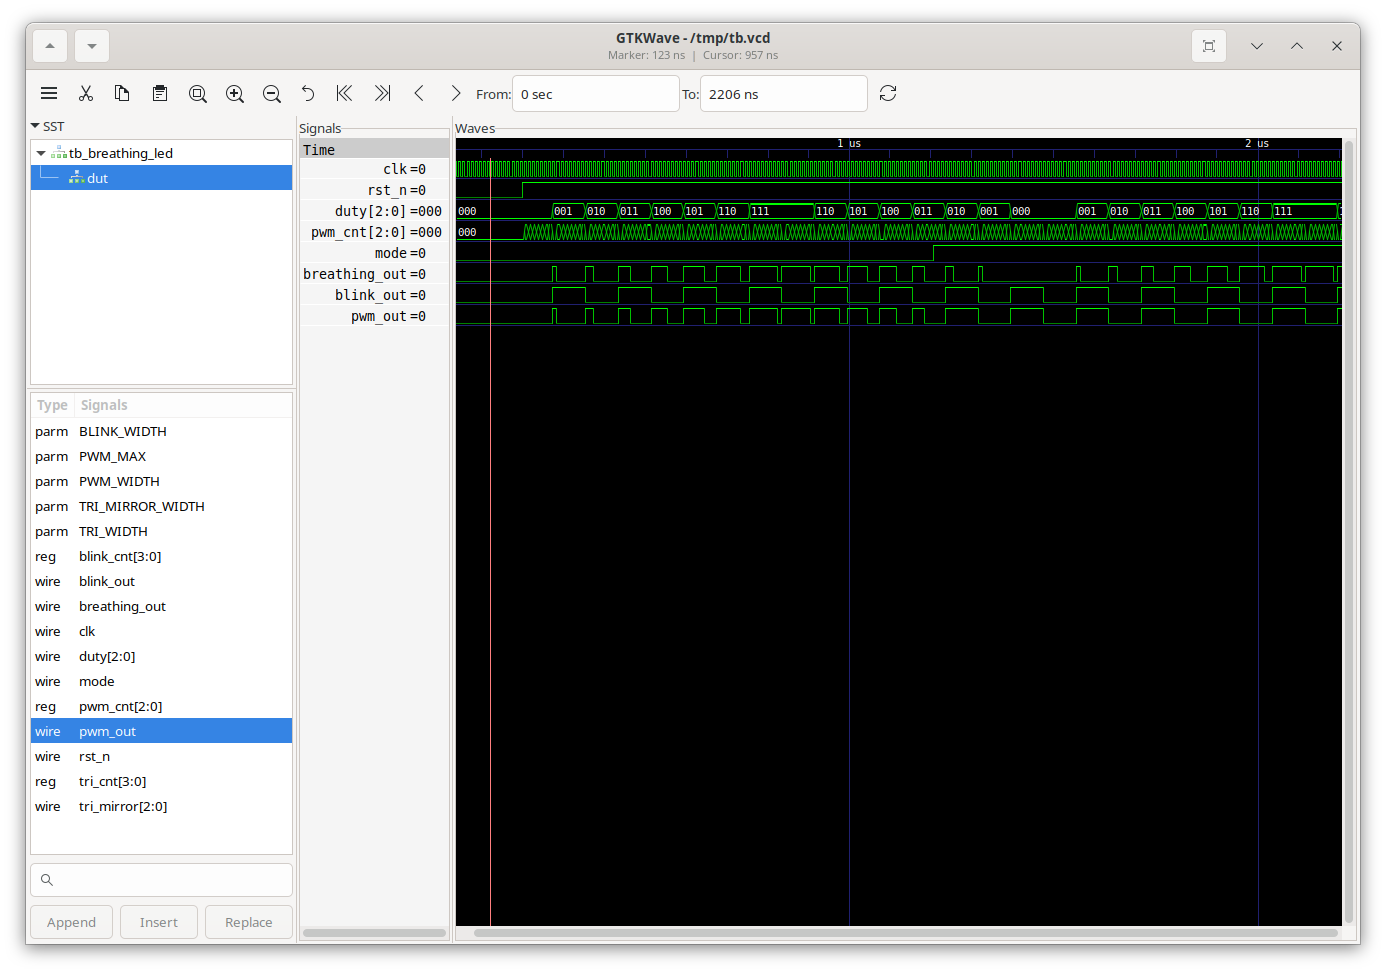
\includegraphics[width=0.95\textwidth]{fig02-gtkwave-screenshot.png}
\end{center}

\textbf{最上面两条：clk 和 rst\_n}

\texttt{clk} 是最密集的绿色波形——它在以固定频率不断翻转，像心跳一样给整个电路提供节奏。\texttt{rst\_n} 则是复位信号，截图左侧它处于低电平（\texttt{0}），表示``系统正在复位''；过了一段时间后跳变为高电平（\texttt{1}），表示``复位释放，系统开始正常运行''。这是一个非常典型的上电时序：先复位，再工作。

\textbf{duty[2:0] 和 pwm\_cnt[2:0]：两个计数器}

\texttt{duty[2:0]} 是三角波计数器。注意它的值从 \texttt{000} 慢慢增加到 \texttt{111}，然后再减回 \texttt{000}，形成一个``爬坡再下坡''的三角形状。这就是``呼吸''的节奏来源——它决定了 PWM 的占空比从最小变到最大，再变回最小。

\texttt{pwm\_cnt[2:0]} 则是快速循环的锯齿波。它的值在 \texttt{000} 到 \texttt{111} 之间反复滚动，速度比 \texttt{duty} 快得多。它是 PWM 的``载波''——就像电台的载波频率远高于音频信号一样，\texttt{pwm\_cnt} 的切换速度也远高于 \texttt{duty} 的变化速度。

\textbf{mode：模式选择开关}

\texttt{mode} 是一个控制信号。为 \texttt{0} 时，系统选择呼吸灯模式；为 \texttt{1} 时，切换到闪烁模式。从截图里可以看到 \texttt{mode} 的变化：在某段时间它是 \texttt{0}，然后跳变为 \texttt{1}，这就解释了为什么后面的波形会发生切换。

\textbf{breathing\_out、blink\_out 和 pwm\_out：三路输出}

\texttt{breathing\_out} 是呼吸灯模式的原始输出——它的脉宽会随着 \texttt{duty} 的变化而变化：\texttt{duty} 大时脉宽宽，\texttt{duty} 小时脉宽窄。\texttt{blink\_out} 则是闪烁模式输出——一个固定频率的方波，与 \texttt{duty} 无关。

\texttt{pwm\_out} 是最终送到 LED 的信号。注意它的行为：\texttt{mode=0} 时，\texttt{pwm\_out} 完全跟随 \texttt{breathing\_out}；\texttt{mode} 变为 \texttt{1} 后，\texttt{pwm\_out} 立刻切换到跟随 \texttt{blink\_out}。这就是一个典型的``二选一''多路选择器在波形上的表现。

\begin{tipbox}
看波形时，不要只看单个信号的形状，更要看\textbf{信号之间的关系}：\texttt{pwm\_out} 为什么变了？是因为 \texttt{mode} 变了。\texttt{breathing\_out} 的脉宽为什么变了？是因为 \texttt{duty} 变了。找到``谁影响谁''的链条，比记住每个信号长什么样更重要。
\end{tipbox}

% ============================================================
\section{综合：从RTL到门级网表}
% ============================================================

\subsection{仿真告诉你「做什么」，综合告诉你「怎么造」}

仿真验证的是行为——在特定输入下，输出是否正确。但它不告诉你：这个设计如果造出来，会用到多少个触发器、多少个逻辑门、它们怎么连接。

综合就是回答这个问题的工具。它读入RTL，经过解析、推断、优化和映射，输出一份\textbf{门级网表}——只包含基本逻辑门（AND、OR、NOT、MUX）和触发器（DFF）的连接关系。

综合器会自动做一些优化，比如把固定不变的信号替换成常量（常量传播）、删除没被用到的逻辑（死代码消除）。这些优化不会改改变电路的外部行为，但会让生成的结构更精简。

\subsection{一条命令完成综合}

\begin{lstlisting}[style=shell]
user@ubuntu:~/projects/lab1$ yosys -p "read_verilog rtl/breathing_led.v; \
    synth -top breathing_led; \
    write_verilog synth/breathing_led_synth.v"
\end{lstlisting}

这条命令做了三件事：读入Verilog文件、以\texttt{breathing\_led}为顶层模块执行综合、把结果写入\texttt{synth/breathing\_led\_synth.v}。

\subsection{网表的``惊喜''}

打开综合后的网表，你会看到类似这样的内容：

\begin{lstlisting}[style=shell]
user@ubuntu:~/projects/lab1$ cat synth/breathing_led_synth.v | head -n 5
$_DFF_PP0_ \tri_cnt_reg[0] (.C(clk), .R(rst_n), .D(...), .Q(...));
$_DFF_PP0_ \tri_cnt_reg[1] (.C(clk), .R(rst_n), .D(...), .Q(...));
$_DFF_PP0_ \tri_cnt_reg[2] (.C(clk), .R(rst_n), .D(...), .Q(...));
$_DFF_PP0_ \tri_cnt_reg[3] (.C(clk), .R(rst_n), .D(...), .Q(...));
$_DFF_PP0_ \tri_cnt_reg[4] (.C(clk), .R(rst_n), .D(...), .Q(...));
\end{lstlisting}

RTL里你写了一个15位的\texttt{tri\_cnt}寄存器，网表里它变成了15个独立的\texttt{\$\_DFF\_PP0\_}单元。组合逻辑（比较器、加法器）则被拆成了\texttt{\$\_AND\_}、\texttt{\$\_OR\_}、\texttt{\$\_MUX\_}等单元的网络。

\begin{tipbox}
你不需要读懂网表里的每一根连线。本章的学习目标只有一个：\textbf{认出RTL里的寄存器在网表里变成了D触发器阵列}。这个对应关系一旦建立，你就理解了``综合不是执行代码，而是把行为翻译成结构''。
\end{tipbox}

\begin{warnbox}
永远不要手动编辑综合后的网表。它是机器生成的，下次综合会被覆盖。永远改RTL源文件。
\end{warnbox}

% ============================================================
\subsection{同一份RTL，两个检查角度}

同一个 \texttt{breathing\_led.v} 文件，Icarus 和 Yosys 都会去读，但你不必在本章就把它们之间全部语义差异吃透。对当前阶段来说，先记住一件更重要的事：\textbf{它们在检查同一个设计的不同侧面。}

\begin{itemize}
  \item \textbf{Icarus（仿真器）}：把 testbench 提供的激励按时间顺序跑一遍，让你观察“这个设计在这些输入下表现如何”。
  \item \textbf{Yosys（综合器）}：把 RTL 映射成寄存器和组合逻辑结构，让你观察“这个设计大致会被实现成什么样子”。
\end{itemize}

所以这里最该建立的判断不是“我已经理解了全部语义细节”，而是：\textbf{仿真回答“它在给定激励下做了什么”，综合回答“它会被组织成什么结构”。} 第二章只要求你先对这两个角度保持警觉，后面章节再系统展开什么样的 RTL 写法会影响综合结果。

\subsection{一个足够说明问题的小例子}

看这段代码（\textbf{不要在真实设计中使用}）：

\begin{lstlisting}[style=shell]
// 危险：缺少 else 分支
always @(*)
  if (condition) out = 1;    // 没有 else！
\end{lstlisting}

你现在不需要在第二章就彻底吃透“为什么这种写法会推断出 latch”的全部语言规则；那是第 4 章要系统讲的内容。本节只需要你先建立一个风险意识：\textbf{RTL 写法如果没有把行为边界交代清楚，综合器就可能生成你本来没打算要的结构。}

对这段代码来说，最朴素的理解已经够用了：\texttt{condition} 为假时，\texttt{out} 该取什么值并没有被清楚说明。仿真里你可能只是看到 \texttt{out} 保持旧值；综合时，工具为了实现这种“保持”的效果，可能会推断出一个锁存器。问题的重点不是你现在就要掌握 latch 的全部细节，而是要记住：\textbf{仿真看起来“能跑”，并不代表结构上就一定符合你的原意。}

这就是为什么第二章要让你同时看波形和综合网表/综合日志，而不是只盯着其中一边。

\begin{warnbox}
\textbf{没有任何验证手段能证明一个设计``绝对正确''——正确永远是条件性的。}

仿真只能证明``在给出的这组激励下，输出没有出错''；综合只能证明``RTL被映射成了这样一组逻辑门''。两者都不保证：
\begin{itemize}
  \item 激励覆盖了所有可能的工作场景
  \item 物理芯片在真实电压、温度和工艺偏差下仍然正确
  \item 设计满足时序、功耗和面积约束
\end{itemize}

所以仿真通过只是起点，不是终点。本章让你同时看波形和网表，是为了建立最基本的警觉：\textbf{行为看起来对，不等于结构一定对；结构看起来对，也不等于物理实现一定对。} 验证是一个逐层收敛的过程，每一层只解决它那一层的问题。
\end{warnbox}

\subsection{验证纪律}

养成这个习惯：
\begin{enumerate}
  \item 写RTL
  \item 仿真，确认波形符合预期
  \item 综合，检查网表和日志中的警告（特别是锁存器推断）
  \item 如果综合报告问题，回改RTL
  \item 两者都通过，才进入下一步（FPGA实现或更高级验证）
\end{enumerate}

% ============================================================
\section{FPGA：可重配置的硬件沙盘}
% ============================================================

\subsection{FPGA是什么，不是什么}

FPGA全称\textbf{现场可编程门阵列}（Field-Programmable Gate Array）。最直白的理解：一块制造完成后还能被重新配置成不同数字电路的芯片。

它\textbf{不是}：
\begin{itemize}
  \item 不是``更灵活的CPU''——CPU执行指令序列，FPGA实现硬件电路
  \item 不是``可编程的逻辑门集合''——它的基本单元是LUT+触发器+互连，不是单个逻辑门
  \item 不是``ASIC的廉价替代品''——在量产场景下，FPGA的单位成本和功耗都高于ASIC
\end{itemize}

它\textbf{是}：
\begin{itemize}
  \item 教学和原型验证的理想平台——可以反复重配置，犯错成本低
  \item 算法加速的灵活载体——某些场景下比CPU/GPU更节能
  \item 小批量系统的可行方案——不需要承担ASIC的流片成本
\end{itemize}

\subsection{FPGA 里面有什么}

想象你有一块巨大的棋盘。每个格子里预先造好了一个小型计算单元。这些单元之间由可编程的``电线''连接。当你下载配置文件到FPGA时，你实际上在做两件事：告诉每个格子``你现在要执行什么逻辑''，以及告诉格子之间的连线``你应该把谁的输出接到谁的输入上''。

下图展示了一个典型FPGA的层次结构：

\begin{center}
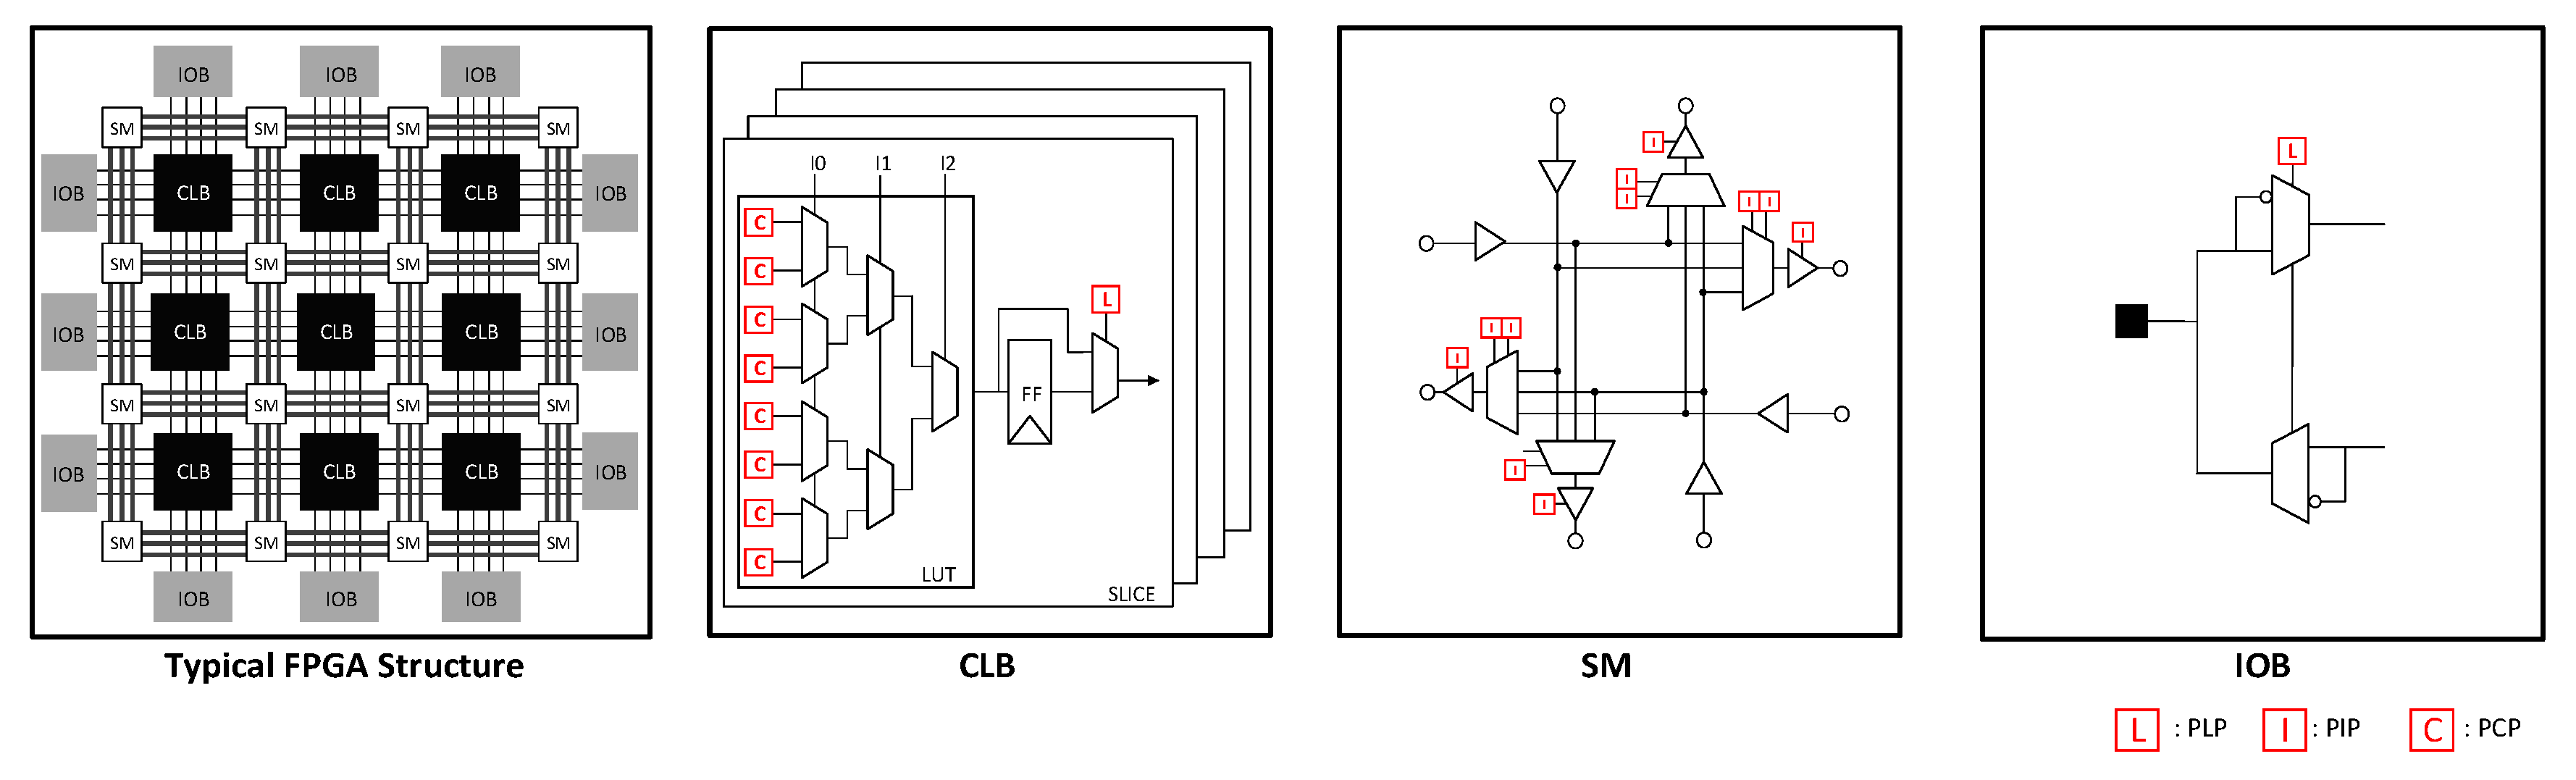
\includegraphics[width=0.95\textwidth]{fig06-fpga-tile.png}
\end{center}

从左到右，这张图呈现了FPGA的三个层次：

\textbf{第一层：整体阵列}（最左）

FPGA的核心是一个二维阵列，阵列中的基本单元叫做CLB（Configurable Logic Block，可配置逻辑块）。阵列的行和列之间穿插着SM（Switch Matrix，开关矩阵）和IOB（I/O Block，输入输出块）。SM负责在CLB之间建立连接，IOB负责把芯片内部的信号引出到外部引脚，或者把外部信号接入芯片内部。

你可以把这个阵列想象成一座城市：CLB是``房子''，SM是``十字路口''，IOB是``城门''。城市里的每栋房子都可以改造成不同的功能（餐厅、办公室、住宅），十字路口决定了哪栋房子和哪栋房子之间有道路连通，城门则负责城市与外界的往来。

\textbf{第二层：CLB 内部}（左起第二）

CLB是FPGA中最核心的计算单元。一个CLB内部通常包含：
\begin{itemize}
  \item \textbf{LUT（查找表）}：实现组合逻辑。图中标记为LUT的部分。一个LUT本质上是一个可配置的真值表——你下载配置时，实际上是在改写这个真值表的内容。比如一个6输入LUT可以实现6个变量的任意布尔函数。它不是``一个逻辑门''，而是``一组逻辑门的集合''。
  \item \textbf{FF（触发器）}：存储状态。图中标记为FF的部分。每个LUT旁边通常配有一个或多个触发器，用于在时钟边沿采样并保存数据。
  \item \textbf{多路选择器}：图中那些三角形带选择端的符号。它们决定信号是走``组合逻辑路径''（直接输出LUT的结果）还是``时序逻辑路径''（经过触发器后再输出）。
  \item \textbf{进位链}：用于高速算术运算（如加法器），把多个LUT串联起来传递进位信号。
\end{itemize}

\textbf{第三层：布线资源}（右起第二和右一）

SM（开关矩阵）和IOB（输入输出块）的细节在图的后两部分展示。SM里布满了可编程开关，这些开关的通断状态由配置比特流决定。IOB则负责信号的电平转换、缓冲和引脚映射——毕竟芯片内部的信号电压和外部电路的电压标准可能不同。

\begin{tipbox}
初学者最容易产生的误解是：以为FPGA里``有一个LUT、一个FF、一根线''，然后这三样东西通过软件组合起来。实际上，FPGA里预先造好了\textbf{成千上万个}LUT、FF、SM和IOB，它们以阵列形式排布在硅片上。你下载的配置文件只决定了：每个LUT的真值表是什么、每个触发器的初始状态是什么、每个开关矩阵的哪些开关闭合。FPGA不是``从无到有''地构造电路，而是``从已有的资源中''选择并连接出你想要的电路。
\end{tipbox}

\subsection{FPGA vs. ASIC}

\begin{center}
\begin{tabular}{lll}
\toprule
\textbf{属性} & \textbf{FPGA} & \textbf{ASIC} \\
\midrule
单位成本 & 较高 & 较低（量产后） \\
首次原型时间 & 分钟 & 数月 \\
功耗效率 & 较低 & 较高 \\
最高时钟频率 & 较低 & 较高 \\
灵活性 & 可重配置 & 流片后固定 \\
\bottomrule
\end{tabular}
\end{center}

教学和原型验证阶段，FPGA赢在\textbf{迭代速度}。写RTL$\rightarrow$综合$\rightarrow$下载到板子，全程几分钟。ASIC的同样流程需要数月和数百万美元。

\subsection{Basys3开发板}

Basys3是教学中最常见的入门级FPGA开发板之一。它的核心是一颗Xilinx Artix-7 FPGA，型号\texttt{xc7a35t-1cpg236c}：
\begin{itemize}
  \item \texttt{xc7a} : Xilinx 7系列Artix家族
  \item \texttt{35} : 约35K逻辑单元
  \item \texttt{t} : 包含高速串行收发器（GTP）
  \item \texttt{-1} : 速度等级（标准）
  \item \texttt{cpg236} : 236引脚封装
  \item \texttt{c} : 商业级温度范围
\end{itemize}

板载外设：16个LED、4位数码管、5个按键、16个拨码开关、USB-UART、VGA、Pmod扩展口。这些外设让实验结果可以直观观察——LED亮灭、按键输入、数码管显示。

\begin{tipbox}
\textbf{Basys3 参考资料}

\url{https://digilent.com/reference/programmable-logic/basys-3/start}

官方页面。另见 Digilent 参考手册（含完整引脚约束和电源规格）。
\end{tipbox}

\begin{center}
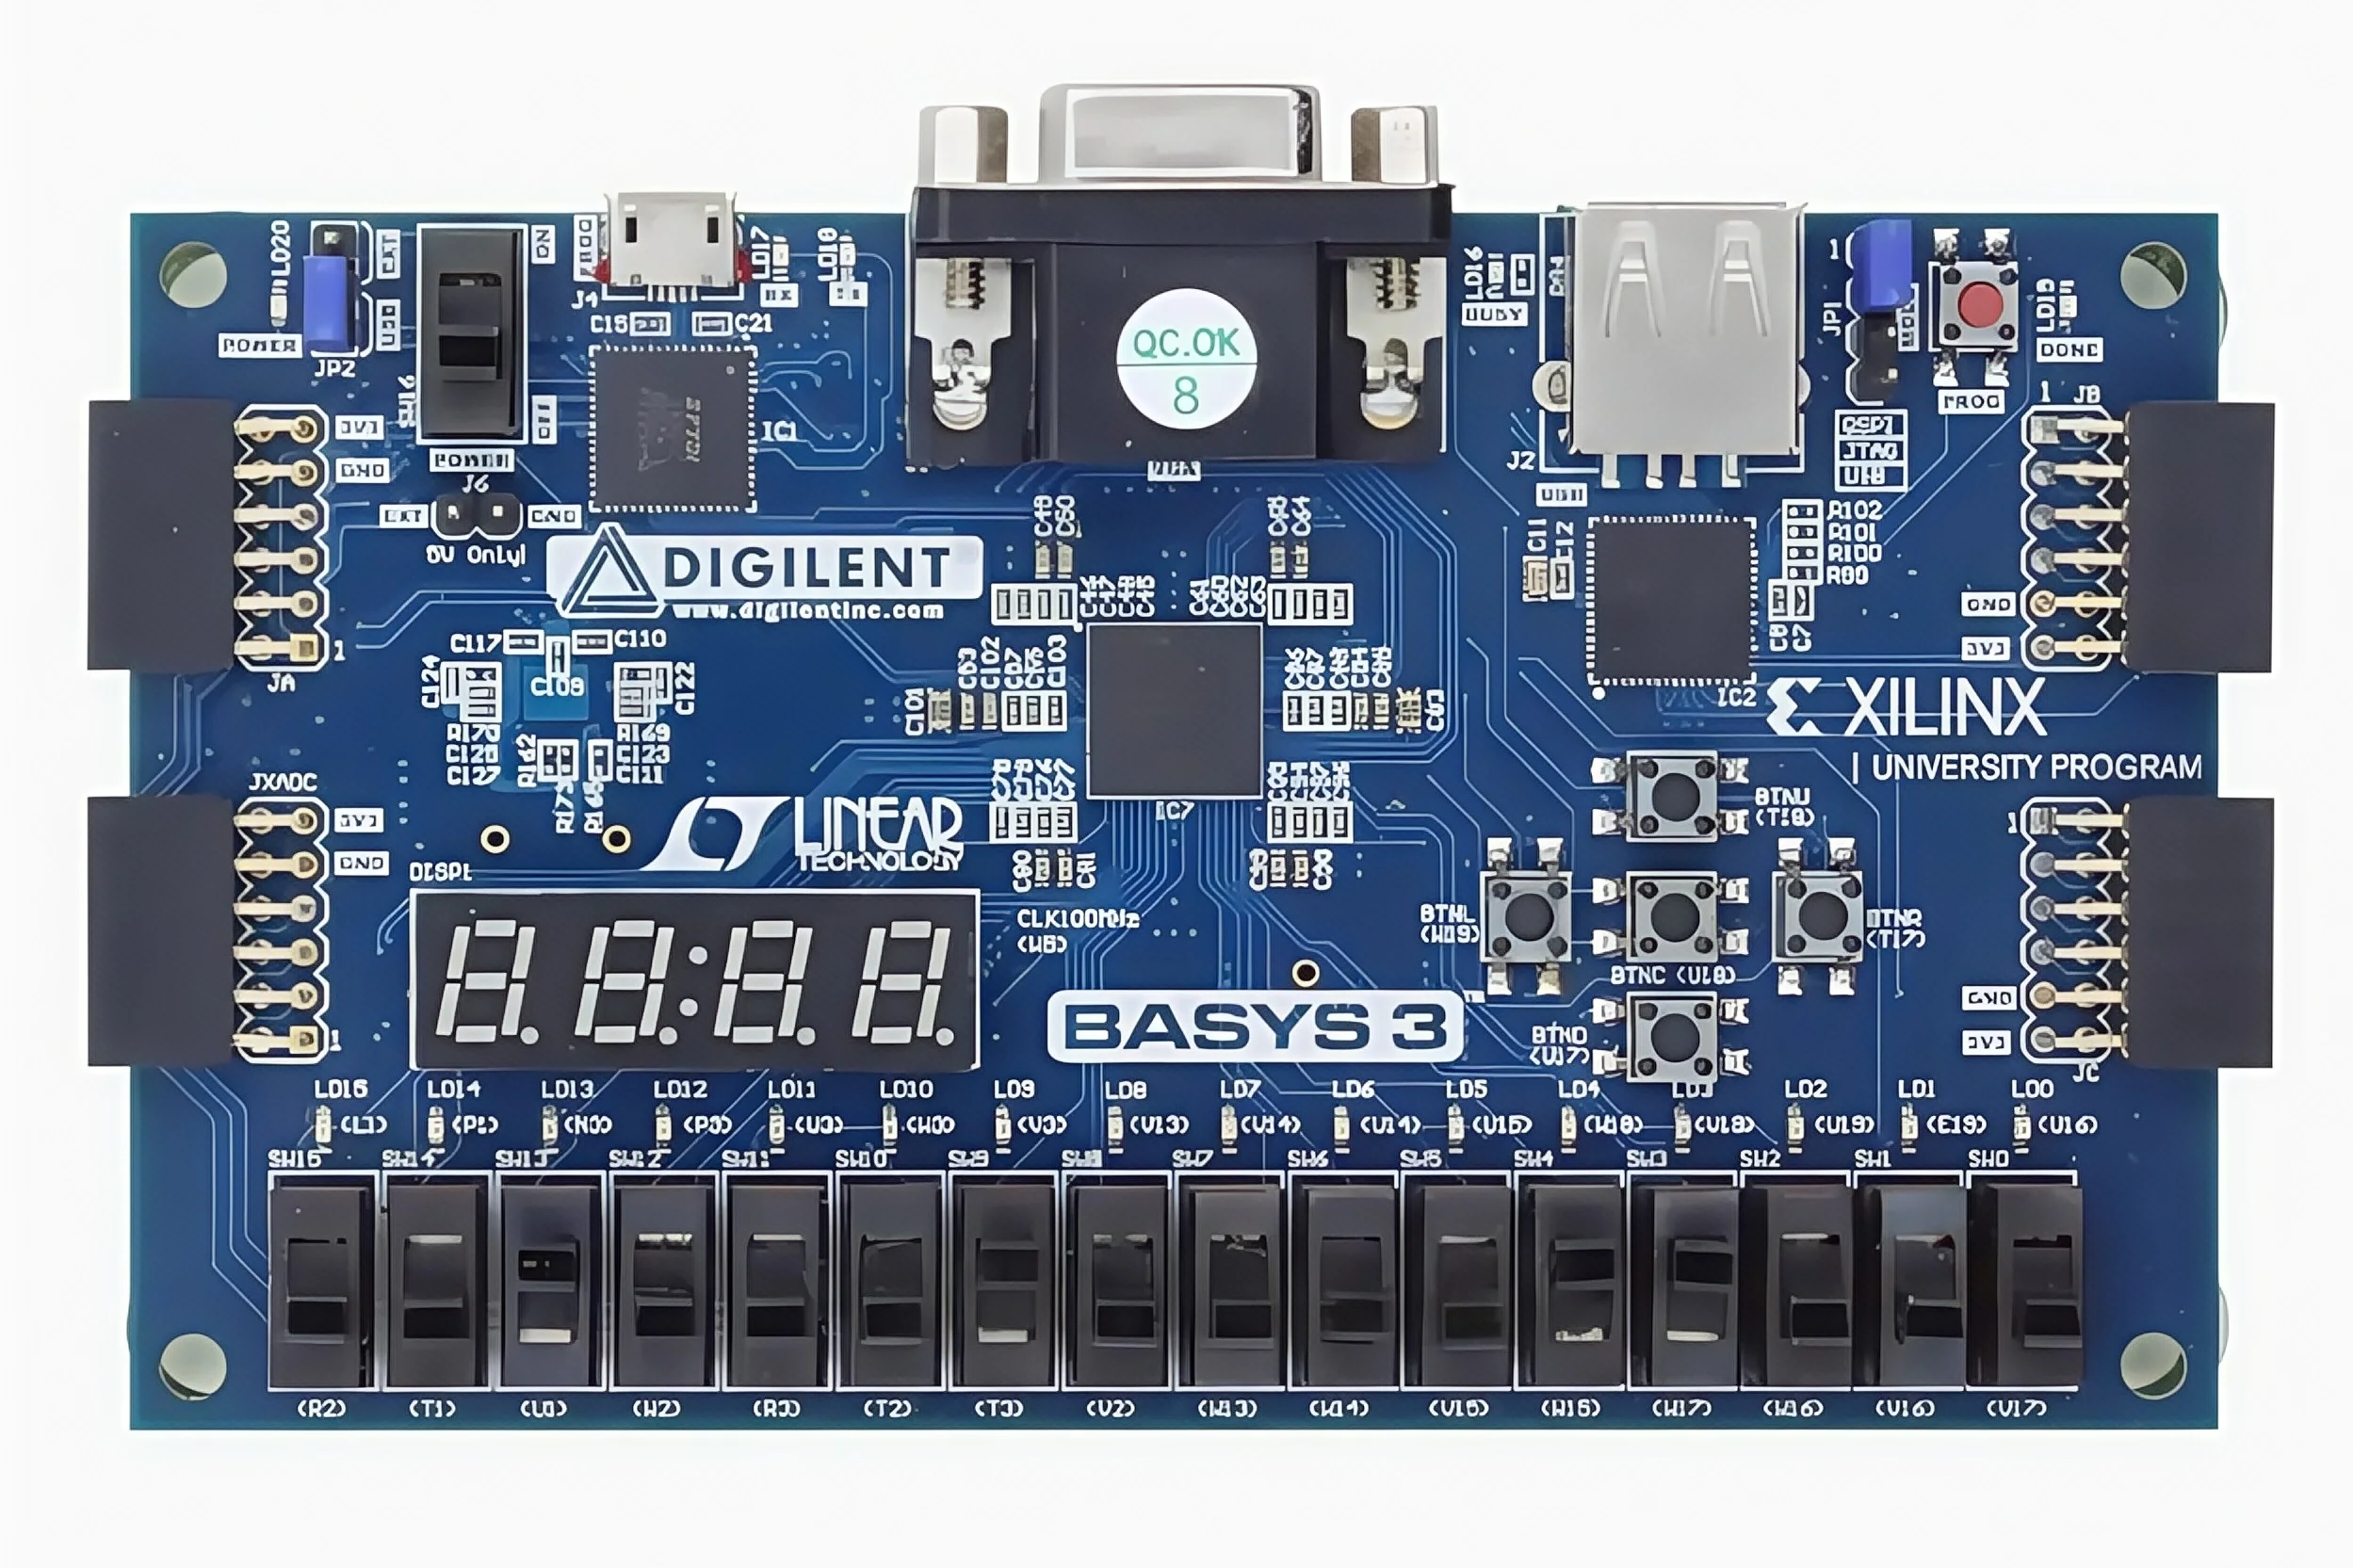
\includegraphics[width=0.75\textwidth]{fig07-basys3-photo.png}
\end{center}

\textbf{Vivado IO Planner}是实现设计时的可视化工具。它把\texttt{cpg236}封装的物理引脚以图形方式展示，你可以把RTL端口（如\texttt{pwm\_out}）拖拽到具体引脚（如LED0），工具自动生成引脚约束。

\begin{center}
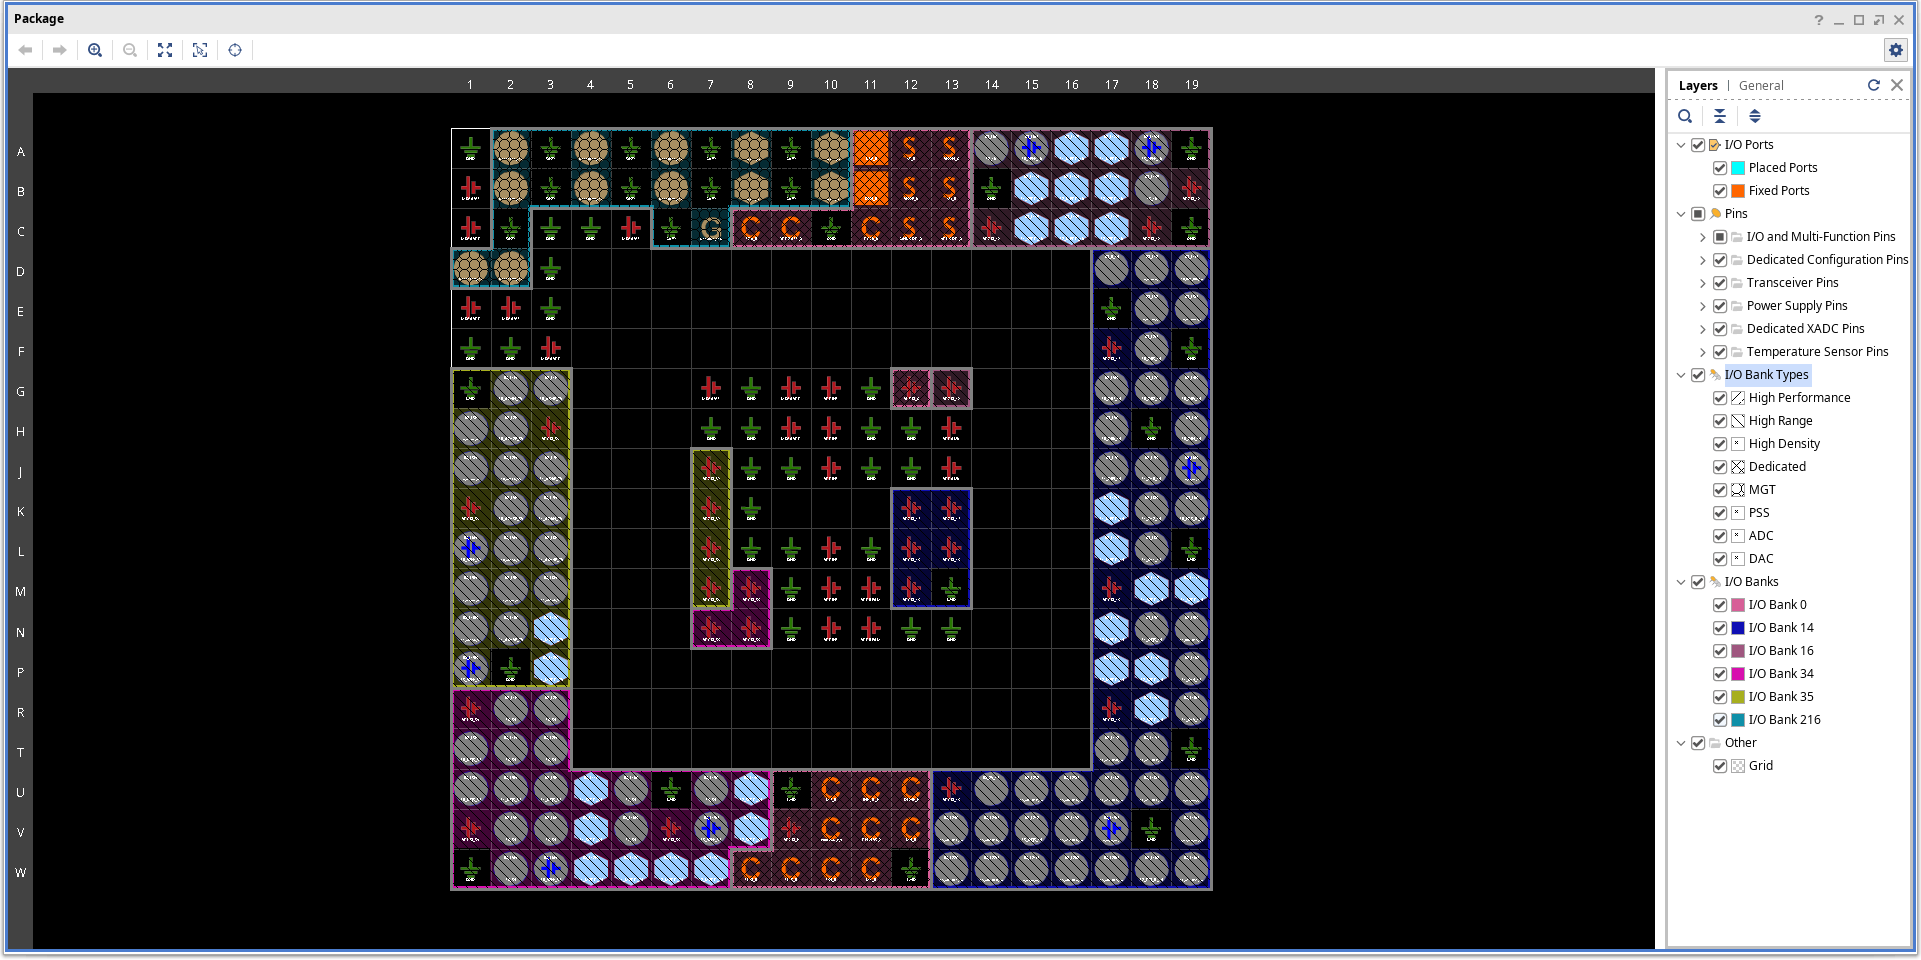
\includegraphics[width=0.85\textwidth]{fig08-vivado-io-planner.png}
\end{center}

\subsection{纯FPGA与SoC FPGA}

Basys3用的是\textbf{纯FPGA}——只有可编程逻辑，没有硬核处理器。在更复杂的系统中，你会遇到\textbf{SoC FPGA}：同一颗芯片上既有ARM处理器（PS，Processing System），又有FPGA fabric（PL，Programmable Logic）。

\begin{center}
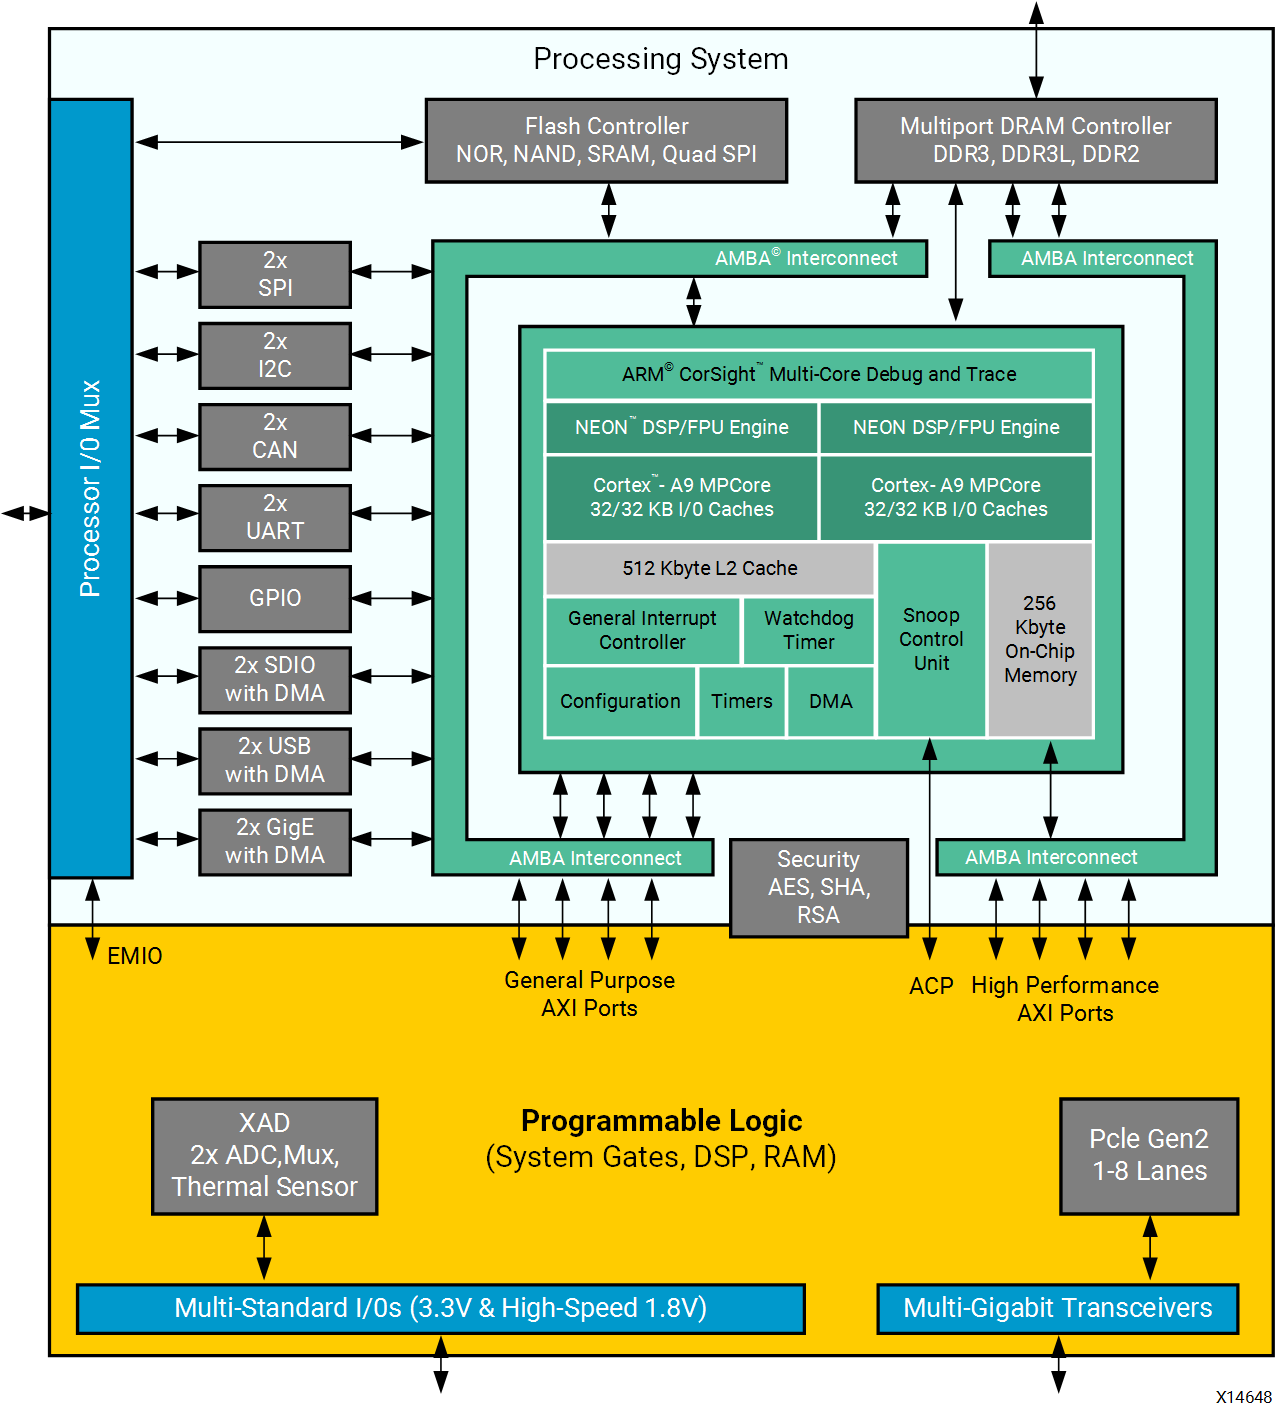
\includegraphics[width=0.85\textwidth]{zynq.png}
\end{center}

上图是Xilinx Zynq-7000架构。ARM Cortex-A9双核CPU运行操作系统和软件，FPGA fabric处理自定义硬件加速。两者通过高速AXI总线通信。这种架构常见于嵌入式系统、软件无线电和硬件加速机器学习。

\begin{tipbox}
知道SoC FPGA存在，能防止``FPGA = 只有逻辑门''的误解。现代FPGA平台是异构系统——纯FPGA（Basys3）是你的起点，但不是终点。
\end{tipbox}

% ============================================================
\section{工具版图：你站在地图的哪个位置}
% ============================================================

\subsection{开源、商业与FPGA厂商：三条线}

数字设计工具不是一条从“低级”到“高级”的直线，而是三条服务于不同约束的工具线。区分它们，是为了知道当前任务需要什么，而不是给工具排身份高低。

\textbf{开源工具线}适合教学、原型验证和可重复实验。它的优势是低门槛、容易安装、命令透明，适合用来建立“RTL如何被仿真、综合和查看”的基本直觉。本章使用的Icarus Verilog、GTKWave和Yosys就属于这一类。

\textbf{商业ASIC工具线}服务于大规模芯片设计和流片签核。它处理的问题包括更大的设计规模、更复杂的时序约束、功耗分析、物理验证、等价检查和工艺库集成。这类工具不是“更漂亮的开源工具”，而是面向工业责任边界的完整系统。

\textbf{FPGA厂商工具线}服务于具体器件。Vivado、Quartus这类工具不仅做综合，还要知道目标芯片里有哪些LUT、触发器、BRAM、DSP、时钟资源和引脚位置。它们的核心任务是把你的RTL落到某一块真实FPGA上，并生成可下载的bitstream。

\begin{center}
\begin{tabular}{llll}
\toprule
\textbf{功能} & \textbf{开源} & \textbf{商业} & \textbf{FPGA厂商} \\
\midrule
仿真 & Icarus Verilog & VCS、Xcelium、Modelsim & Vivado Simulator \\
波形 & GTKWave & SimVision、Verdi & Vivado Simulator \\
综合 & Yosys & Design Compiler、Genus & Vivado Synthesis \\
Lint/CDC & Verilator（部分） & SpyGlass、Conformal & --- \\
布局布线 & nextpnr、OpenROAD & ICC2、Innovus & Vivado Implementation \\
\bottomrule
\end{tabular}
\end{center}

所以，本章选择开源工具不是因为它“代表全部工业流程”，而是因为它足够小、足够透明，适合看清第一条闭环：写RTL、跑仿真、看波形、做综合。后面真正上FPGA时，我们会进入厂商工具；如果未来走向ASIC流片，还会进入商业签核流程。三条线不是互相鄙视的阵营，而是不同阶段、不同风险、不同成本下的工程选择。

\subsection{商业工具链长什么样}

为了给你具体的感知，下面是Cadence的数字全流程。这不是本章要用的工具，但它是你在工业界或高级研究中会遇到的。

\begin{center}
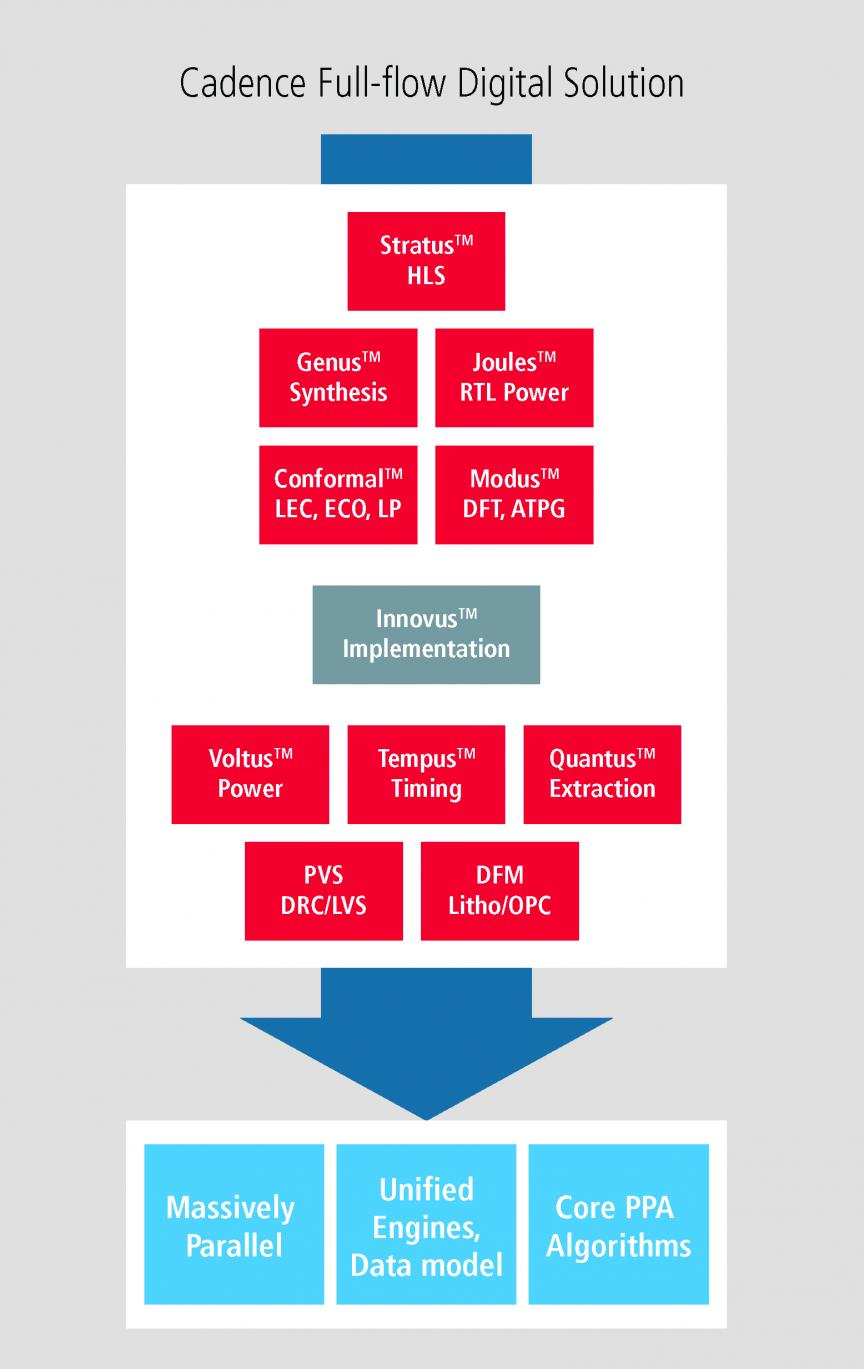
\includegraphics[width=0.50\textwidth]{cadence-toolkit.jpg}
\end{center}

\textbf{自上而下：}
\begin{enumerate}
  \item \textbf{Stratus HLS} : 高层次综合，把C/C++转成RTL
  \item \textbf{Genus} : RTL综合
  \item \textbf{Joules} : RTL功耗分析
  \item \textbf{Conformal} : 逻辑等价检查、低功耗验证
  \item \textbf{Modus} : 可测试性设计、自动测试向量生成
  \item \textbf{Innovus} : 布局布线、时序优化
  \item \textbf{Voltus / Tempus / Quantus} : 功耗、时序、寄生参数签核
  \item \textbf{PVS / DFM} : 物理验证（设计规则检查、版图vs电路图）
\end{enumerate}

每个工具都需要单独license和集成。你本章学的开源工具链（Icarus + GTKWave + Yosys）只覆盖了\textbf{仿真和综合}两层——但这正是学习和原型验证所需的最小集合。

\begin{warnbox}
商业流程不是``更好的开源''。它是在不同约束（更大规模、更先进工艺、更高可靠性要求）下的不同解决方案。先学会用开源工具建立直觉，再根据需要迁移到商业工具——这个顺序更合理。
\end{warnbox}

% ============================================================
\section{补充：Makefile与FPGA上板}
% ============================================================

前面已经分别讲过仿真、波形、综合和FPGA的基本概念，这里不再重复完整流程。本节只补充两个实际工程入口：用Makefile统一命令，以及在Basys3上下载验证。

\subsection{为什么需要Makefile}

同一个实验通常会反复执行几类操作：编译仿真、打开波形、运行综合、生成bitstream、下载到板子、清理生成文件。如果每次都手敲完整命令，不仅麻烦，也容易因为目录或参数写错而制造无关错误。

Makefile的作用是把这些固定流程收进几个稳定入口：

\begin{lstlisting}[style=shell]
$ make sim          # 编译 + 仿真 + 打开GTKWave
$ make synth        # 运行Yosys综合
$ make fpga         # 生成比特流（需要Vivado）
$ make program      # 下载到板子（需要Vivado + Basys3）
$ make clean        # 清理生成文件
\end{lstlisting}

这不是新的工具链，而是对前面命令的封装。你可以先用 \texttt{make sim} 快速确认环境可用；如果想看清细节，再打开 \texttt{sim/run.sh}、\texttt{synth/run.sh} 或 \texttt{fpga/run.tcl}，逐行对照前面讲过的工具角色。

\begin{tipbox}
Makefile适合保存“已经确定下来的流程”。调试命令时可以手动执行；流程稳定后，再把它收进Makefile，减少重复劳动和手误。
\end{tipbox}

\subsection{FPGA上板验证}

仿真和综合都通过后，如果你手边有Basys3开发板和Vivado，可以把设计真正下载到FPGA上。进入实验目录后执行：

\begin{lstlisting}[style=shell]
user@ubuntu:~/examples/lab1-breathing-led$ make fpga
=== 生成比特流（2-3分钟） ===
...
user@ubuntu:~/examples/lab1-breathing-led$ make program
=== 下载到板子 ===
...
\end{lstlisting}

下载完成后，LED0会显示呼吸效果。按BTNR切换到闪烁模式，再按一次切回呼吸模式；按BTNC复位电路。

\begin{warnbox}
FPGA上板比仿真多了两个前提：一是Vivado路径正确，二是开发板通过USB连接并被系统识别。Vivado默认路径是 \texttt{/opt/Xilinx/Vivado/2019.2/bin/vivado}；如果安装位置不同，需要修改Makefile中的 \texttt{VIVADO} 变量。
\end{warnbox}

\subsection{清理生成文件}

实验过程中会产生 \texttt{*.vcd}、\texttt{*.vvp}、\texttt{*\_synth.v}、Vivado工程中间文件等生成物。需要恢复干净目录时执行：

\begin{lstlisting}[style=shell]
user@ubuntu:~/examples/lab1-breathing-led$ make clean
=== 删除生成文件 ===
\end{lstlisting}

清理命令只删除生成文件，保留RTL源码、testbench、约束文件、脚本和Makefile。

% ============================================================
\section{本章总结}
% ============================================================

本章要点：

\begin{itemize}
  \item \textbf{Linux命令行}是更适合工程重复性与可复现性的工作台，不是GUI的``高级版''
  \item \textbf{仿真}验证行为，\textbf{综合}产出结构，两者都必须检查
  \item \textbf{波形}是主要调试窗口——学会读时间、边沿、X/Z和占空比
  \item \textbf{开源工具}（Icarus、GTKWave、Yosys）构成完整的学习工具链
  \item \textbf{FPGA}把验证闭环焊死在真实硬件上
\end{itemize}

\textbf{这为后续章节提供了什么：}
\begin{itemize}
  \item 第三章（组合逻辑）：每个门都可以写RTL$\rightarrow$仿真$\rightarrow$看波形
  \item 第四章（Verilog HDL）：你已经会编译和仿真，现在只需学语言
  \item 第七章（系统级RTL）：复用同样的项目结构和工具脚本
\end{itemize}

% ============================================================
\section{术语表}
% ============================================================

\begin{center}
\begin{tabular}{lp{10cm}}
\toprule
\textbf{术语} & \textbf{定义} \\
\midrule
RTL & Register Transfer Level，寄存器传输级。用寄存器和组合逻辑描述硬件行为。 \\
Testbench & 仿真用的验证代码，为DUT提供激励并检查输出。 \\
Icarus Verilog & 开源Verilog仿真器。 \\
GTKWave & 开源波形查看器，读取VCD等波形格式。 \\
Yosys & 开源RTL综合工具，将RTL转换为门级网表。 \\
VCD & Value Change Dump，波形文件格式。 \\
VVP & Icarus Verilog的运行时引擎。 \\
Netlist & 网表——描述逻辑门及其连接关系的文件。 \\
LUT & Look-Up Table，FPGA中实现组合逻辑的基本单元。 \\
FF & Flip-Flop，触发器，FPGA中实现时序逻辑的基本单元。 \\
PWM & Pulse Width Modulation，脉冲宽度调制。 \\
Duty Cycle & 占空比，PWM波形中高电平时间占总周期的比例。 \\
\bottomrule
\end{tabular}
\end{center}

% ============================================================
\section{练习题}
% ============================================================

\begin{enumerate}
  \item \textbf{工具安装证明}\\
  安装Icarus Verilog、GTKWave和Yosys，在本地电脑上完成复现本章样例所需的最小环境配置。

  \item \textbf{跑通完整闭环}\\
  进入 \texttt{examples/lab1-breathing-led/}，执行 \texttt{bash sim/run.sh} 和 \texttt{bash synth/run.sh}。通过GTKWave查看\texttt{duty}、\texttt{pwm\_cnt}、\texttt{pwm\_out}的波形，解释三角波与PWM输出的关系。

  \item \textbf{检查网表}\\
  打开 \texttt{synth/breathing\_led\_synth.v}，定位\texttt{tri\_cnt}对应的触发器。单元名是什么？（提示：搜索 \texttt{\$\_DFF}。）

  \item \textbf{参数探索}\\
  把 \texttt{TRI\_WIDTH} 从15改为13，重新仿真。占空比变化周期发生了什么？为什么？

  \item \textbf{Why/What/How分析Yosys}\\
  从``为什么需要综合器''（Why）、``综合器做什么''（What）、``怎么用Yosys''（How）三个维度分析Yosys，并对比仿真器和综合器的区别。

  \item \textbf{反转比较器}\\
  修改比较逻辑让LED在计数器值小时亮。仿真确认波形变化。这在物理板上意味着什么？

  \item \textbf{开源工具调研（选做）}\\
  搜索一个本章未涉及的开源工具（OpenROAD、F4PGA、Verilator、Cocotb等），说明它做什么、对应本章哪个工具、强在哪/弱在哪。
\end{enumerate}

\end{document}
